% Wireframe previo del layout global (análisis de diseño)
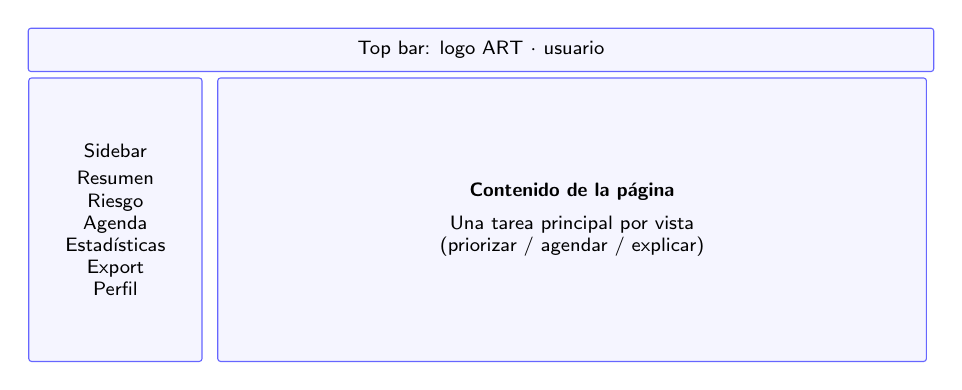
\begin{tikzpicture}[
  font=\scriptsize\sffamily,
  box/.style={draw=blue!60, fill=blue!4, rounded corners=1pt, align=center},
  ]
  \node[box, minimum width=11.5cm, minimum height=0.55cm] (top) at (0,3.2)
    {Top bar: logo ART $\cdot$ usuario};
  \node[box, minimum width=2.2cm, minimum height=3.6cm, anchor=north west] (side) at (-5.75,2.85)
    {Sidebar\\[2pt]Resumen\\Riesgo\\Agenda\\Estad\'isticas\\Export\\Perfil};
  \node[box, minimum width=9.0cm, minimum height=3.6cm, anchor=north west] (main) at (-3.35,2.85)
    {\textbf{Contenido de la p\'agina}\\[4pt]
     Una tarea principal por vista\\
     (priorizar / agendar / explicar)};
\end{tikzpicture}
